\section{Regelung}

\textbf{Regelungstechnik}: Lehre von der selbsttätigen, gezielten Beeinflussung dynamischer Prozesse während des Prozessablaufs bei unvollständiger Systemkenntnis, insbesondere bei Störungen
\begin{center}
	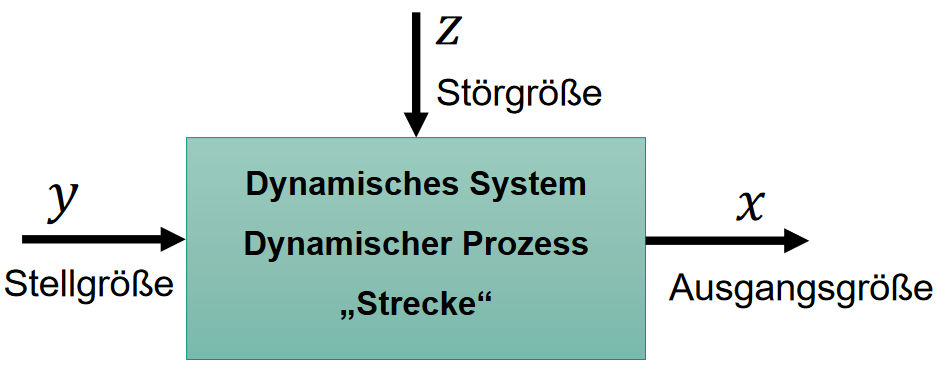
\includegraphics[width=0.4\textwidth]{images/regelung.png}
\end{center}

\textbf{Aufgabe}: Ausgangsgröße eines dynamischen Systems soll mittels der Stellgröße ein
Sollverhalten gegen den Einfluss einer Störgröße aufzeigen



